\documentclass[preprint,12pt]{elsarticle}
\usepackage[utf8]{inputenc}
\usepackage{amssymb,amsmath,amsfonts,amsthm}
\usepackage{tikz}
\usepackage{xcolor}

\newcommand{\Ec}{\mathcal{E}}

\newcommand{\Dc}{\mathcal{D}}

\newcommand{\Rc}{\mathcal{R}}

\newcommand{\Pc}{\mathcal{P}}

\newcommand{\Ac}{\mathcal{A}}

\newcommand{\Gdex}{\mathcal{G}^{\dagger}_{\text{ext}}}

\newcommand{\Rb}{\mathbb{R}}

\newcommand{\Hb}{\mathbb{H}}

\begin{document}

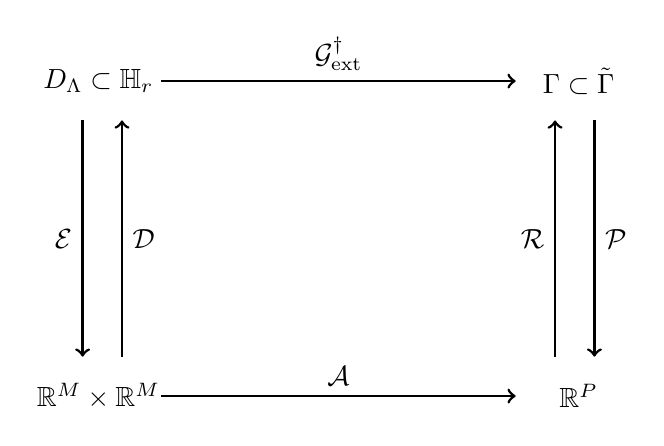
\begin{tikzpicture}
    % Define line width for bold arrows
    \tikzset{boldarrow/.style={->, line width=1.0pt}}

    % Parallel to y-axis arrows
    \draw[boldarrow] (0.0,3) to node[left] {$\Ec$} (0.0,0);
    \draw[boldarrow] (0.5,0) to node[right] {$\Dc$} (0.5,3);
    
    \draw[boldarrow] (6.0,0) to node[left] {$\Rc$} (6.0,3);
    \draw[boldarrow] (6.5,3) to node[right] {$\Pc$} (6.5,0);
    
    % Parallel to x-axis arrows
    \draw[boldarrow] (1.0,-0.5) to node[above] {$\Ac$} (5.5,-0.5);
    \draw[boldarrow] (1.0,3.5) to node[above] {$\Gdex$} (5.5,3.5);
    
    % Labels 
    \draw node at (0.2,-0.5) {$\mathbb{R}^{M}\times \Rb^M$};
    \draw node at (0.2,3.5) {$D_{\Lambda}\subset\Hb_r$};
    \draw node at (6.3,-0.5) {$\mathbb{R}^{P}$};
    \draw node at (6.3,3.5) {$\Gamma\subset\tilde{\Gamma}$};
\end{tikzpicture}

\end{document}